\documentclass[tikz]{standalone}
\usepackage{pgfplots}
\pgfplotsset{compat=1.15}
\usepackage{mathrsfs}
\usetikzlibrary{arrows,calc}
\usepackage{tkz-euclide}
\pagestyle{empty}

\definecolor{uuuuuu}{rgb}{0.26666666666666666,0.26666666666666666,0.26666666666666666}
\definecolor{AngleClr}{rgb}{0,0.39215686274509803,0}
\definecolor{ShapeClr}{rgb}{0.6,0.2,0}
\definecolor{SquareClr}{RGB}{250, 248, 217}

\usepackage{fp}
\usepackage{xfp}

\begin{document}

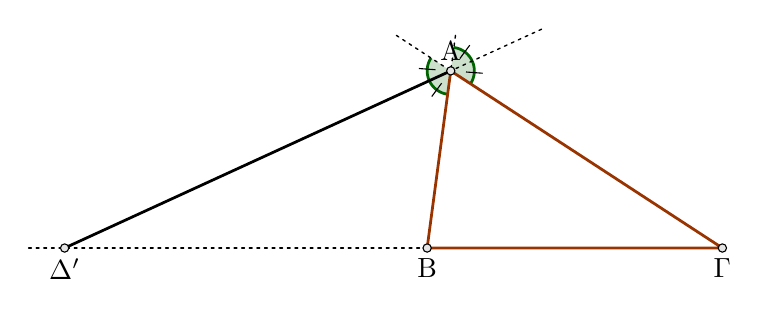
\begin{tikzpicture}[scale=.75]
\tkzSetUpLine[line width=1pt,color=black]

\tkzDefPoints{0/0/B,0.4/3/A,5/0/C}


% \tkzDefPointBy[projection=onto B--C](A)\tkzGetPoint{H}

\tkzDefPointOnLine[pos=-0.2](A,C) \tkzGetPoint{C'}
\tkzDefPointOnLine[pos=-0.2](A,B) \tkzGetPoint{B'}

\tkzDefLine[bisector out](C,A,B) \tkzGetPoint{x}
\tkzInterLL(A,x)(B,C) \tkzGetPoint{D}

\tkzDefPointOnLine[pos=1.2](D,A)\tkzGetPoint{E}

\tkzFillPolygon[fill=white](A,B,C)
% \tkzMarkRightAngle[line width=1pt, size=.35,color=AngleClr,fill=AngleClr,fill opacity=0.1](B,A,C)
% \tkzFillAngle[fill=AngleClr,size=.4,fill opacity=0.1](A,C,B)
% \tkzMarkAngle[line width=1pt,color=AngleClr,size=.4](A,C,B)
% \tkzFillAngle[fill=AngleClr,size=.4,fill opacity=0.1](B',A,C)
% \tkzMarkAngle[line width=1pt,color=AngleClr,size=.4](B',A,C)
% \tkzMarkRightAngle[line width=1pt, size=.2,color=AngleClr,fill=AngleClr,fill opacity=0.1](A,H,B')

\tkzFillAngle[fill=AngleClr,size=.4,fill opacity=0.2](D,A,B)
\tkzMarkAngle[line width=1pt,size=.4,color=AngleClr,mark=|,mksize=3](D,A,B)

\tkzFillAngle[fill=AngleClr,size=.4,fill opacity=0.2](C',A,D)
\tkzMarkAngle[line width=1pt,size=.4,color=AngleClr,mark=|,mksize=3](C',A,D)

\tkzFillAngle[fill=AngleClr,size=.4,fill opacity=0.2](C,A,E)
\tkzMarkAngle[line width=1pt,size=.4,color=AngleClr,mark=|,mksize=3](C,A,E)

\tkzFillAngle[fill=AngleClr,size=.4,fill opacity=0.2](E,A,B')
\tkzMarkAngle[line width=1pt,size=.4,color=AngleClr,mark=|,mksize=3](E,A,B')


\tkzDrawSegment[line width=0.5pt,color=black,dashed,dash pattern=on 1pt off 1.75pt,add=0 and 0.1](B,D)
\tkzDrawLine[line width=0.5pt,color=black,dashed,dash pattern=on 1pt off 1.75pt,add=.2 and 0](A,C)
\tkzDrawLine[line width=0.5pt,color=black,dashed,dash pattern=on 1pt off 1.75pt,add=.2 and 0](A,B)
\tkzDrawLine[line width=0.5pt,color=black,dashed,dash pattern=on 1pt off 1.75pt](A,E)
\tkzDrawSegment[line width=1pt](A,D)

\tkzDrawPolygon[color=ShapeClr](A,B,C)

\tkzDrawPoints[size=3](A,B,C,D)



% \tkzDrawSegment[line width=0.5pt,color=black,dashed,dash pattern=on 1pt off 1.75pt](H,B')


\tkzLabelPoint[above](A){$\mathrm{A}$}
\tkzLabelPoint[below](D){$\mathrm{\Delta}'$}
% \tkzLabelPoint[left](B){$\mathrm{B}'$}
\tkzLabelPoint[below](B){$\mathrm{B}$}
\tkzLabelPoint[below](C){$\mathrm{\Gamma}$}

\end{tikzpicture}

\end{document}
